%% History:
% Ondrej Guth (2022-03-22)
% Josef Hlavac & Tomas Zahradnicky (4.10.2010)
%  + Built on the FEL CVUT template by Daniel Sykora and Pavel Tvrdik
%  + Made for FIT CVUT
%  + Joined several chapters and cleaned
%  + Undefined references are typeset in an orange box to alert the writer!
%  + Index is automatically printed if the \usepackage{index} and
%    \newindex{default}{idx}{ind}{Index} lines are uncommented.
%
\documentclass[12pt,twoside,a4paper,final]{memoir}%two-page printing

\usepackage{a4wide}

%\usepackage[T1]{fontenc}
% \usepackage[czech,english]{babel}
\usepackage{graphicx}
\usepackage{pdflscape}
%\usepackage{setspace}
%\usepackage{epic} % Images drawn in Xfig, exported as .epic

\usepackage{hyperref}
% \usepackage[hidelinks]{hyperref} %hyperlinks without colour boxes
% \usepackage[usenames]{color}
\usepackage{amssymb}
\usepackage{amsmath}
\usepackage{amsthm}

% \usepackage{tikz}
\usepackage[chapter]{algorithm}
% \usepackage{algpseudocode}
% \renewcommand{\algorithmicrequire}{\textbf{Input:}}
% \renewcommand{\algorithmicensure}{\textbf{Output:}}

%\usepackage{proof}
%\usepackage{latexsym}
% \usepackage{rotating}
%\usepackage{epsfig}
% \usepackage{subfigure}
% \usepackage{multirow}
%\usepackage{index}
%\newindex{default}{idx}{ind}{Index}

\usepackage[
nonumberlist, %do not show page numbers
acronym,      %generate acronym listing   -> Not used in this example (see line with %%% )
nomain,
numberedsection
% notoc,          %show listings as entries in table of contents
]      %use section level for toc entries
{glossaries}
\makeglossaries
\input tex/phdmacro.tex %couple of macros for formatting the dissertation thesis,
                    %your personal and specific macros can be placed also there


\renewcommand{\labelitemi}{\(\circ\)}

\newenvironment{chapterintro}{\slshape}{\par}

\usepackage{etoolbox}
% fix TOC in memoir class
\makeatletter
\renewcommand{\@pnumwidth}{2em} 
\renewcommand{\@tocrmarg}{3em}
\patchcmd{\@endtheorem}{\@endpefalse}{}{}{}
\patchcmd{\endproof}{\@endpefalse}{}{}{}
\makeatother

\newcommand\DissTitle{DISSERTATION THESIS TITLE}
\newcommand\FirstandFamilyName{YOUR NAME}
\newcommand\Email{USERNAME@fit.cvut.cz}
\newcommand\Month{Prague, August}
\newcommand\Year{2022}
\newcommand\Supervisor{prof. PETER SUPERVISOR, Ph.D.}
\newcommand\SupervisorAffiliation{
Department of Theoretical Computer Science\\
%Department of Digital Design\\
%Department of Software Engineering\\
% Department of Computer Systems\\
Faculty of Information Technology\\
Czech Technical University in Prague\\
Th\'akurova 9\\
160 00 Prague 6\\
Czech Republic}
%%-> uncomment if you have a thesis co-supervisor
%\newcommand\CoSupervisor{prof. RNDr. COSUPERVISOR, Ph.D.}
%\newcommand\CoSupervisorAffiliation{
%Computer Science and Engineering Department\\
%Faculty of Electrical Engineering\\
%Czech Technical University in Prague\\
%Karlovo n\'{a}m.~13\\
%121 35 Prague 2\\
%Czech Republic}

\newcommand\PhDProgram{Informatics}
%\newcommand\PhDSpecialization{Informatics}
\newcommand\Department{Department of Theoretical Computer Science}
%\newcommand\Department{Department of Digital Design}
%\newcommand\Department{Department of Software Engineering}
% \newcommand\Department{Department of Computer Systems}
\newcommand\Faculty{Faculty of Information Technology}
\newcommand\University{Czech Technical University in Prague}
\newcommand\Address{Th\'akurova 9, 160 00 Prague 6, Czech Republic}

\def\UrlBreaks{\do\/\do\-}



\newacronym{DFA}{DFA}{deterministic finite automaton}
\newacronym{NFA}{NFA}{nondeterministic finite automaton}
\newacronym{FA}{FA}{finite automaton}

\maxsecnumdepth{subsubsection}
\setcounter{tocdepth}{2}
\makeheadstyles{FITthesis}{
	\chapterstyle{madsen}
	\setsecheadstyle{\Large\bfseries\sffamily}
	\setsubsecheadstyle{\large\bfseries\sffamily}
	\setsubsubsecheadstyle{\bfseries\sffamily}
}
\headstyles{FITthesis}

% \includeonly{
% 	tex/abstract
% 	,tex/acknowledgement
% 	,tex/introduction
% 	,tex/stateoftheart
% 	,tex/conclusions
% }

\begin{document}

\theoremstyle{definition}
\newtheorem{lemma}{Lemma}[section]
\newtheorem{theorem}[lemma]{Theorem}
\newtheorem{definition}[lemma]{Definition}
\newtheorem{preposition}[lemma]{Preposition}
\newtheorem{example}[lemma]{Example}
\newtheorem{corollary}[lemma]{Corollary}
\newtheorem{proposition}[lemma]{Proposition}
\newtheorem{property}[lemma]{Property}
\newtheorem{observation}[lemma]{Observation}
\theoremstyle{remark}
\newtheorem{notation}[lemma]{Notation}
\newtheorem{note}[lemma]{Note}

% allow @ to appear in macro names
% \makeatletter

% % produce undefined references in an orange box rather than just ??
% \def\@setref#1#2#3{%
%   \ifx#1\relax
%    \protect\G@refundefinedtrue
%    \nfss@text{\reset@font\bfseries\fcolorbox{black}{Orange}{??}}%
%    \@latex@warning{Reference `#3' on page \thepage \space
%              undefined}%
%   \else
%    \expandafter#2#1\null
%   \fi}


\frontmatter
\openany

\coverpagestarts

\pagestyle{ruled}

\chapter*{Abstract and contributions}
%\addcontentsline{toc}{chapter}{\protect\numberline{}{Abstract and contributions}}

This \thesis{} deals with \dots 


\bigskip
\noindent In particular, the main contributions of the \thesis{} are as follows:
\begin{enumerate}
\item
Design of a methodology of a \dots

\item
\dots

\item
\dots
\end{enumerate}


\bigskip

\noindent\textbf{Keywords:}

~keyword1, keyword2, keyword3, keyword4, keyword5.

\vfill
%If you present in this thesis work achieved jointly with some other people except for your supervisor or co-supervisor, then this is a place to put their statements clarifying your qualitative and quantitative participation.
%For example,

%\noindent As a collaborator of {\FirstandFamilyName} and a co-author of his papers, I agree with {\FirstandFamilyName}'s authorship of the research results, as stated in this dissertation thesis.

%\bigskip\bigskip
%\begin{flushright}
%    \begin{tabular}{p{6cm}}
%           \dotfill\\
%           {\em Name Surname}
%    \end{tabular}
%\end{flushright}

\chapter*{Abstrakt}

% \selectlanguage{czech}

Abstrakt v {\v c}esk{\'e}m jazyce je povinnou sou{\v c}{\'a}st{\'i} práce.

\noindent\textbf{Kl{\'i}{\v c}ov{\'a} slova:}

~kl{\'i}{\v c}ov{\'e} slovo 1, kl{\'i}{\v c}ov{\'e} slovo 2.

% \selectlanguage{english}


% \newpage
\chapter*{Acknowledgements}

First of all, I would like to express my gratitude to my dissertation thesis
supervisor, Dr. R\'obert~L\'orencz. He~has been a constant source of encouragement and insight during my research and helped me with numerous problems and professional advancements.  

I would like to thank to Dr. \dots, and Prof. \dots for giving me \dots

Special thanks go to the staff of the \Department{}, who maintained a pleasant and flexible environment for my research. I would like to express special thanks to the department management for providing most of the funding for my research. 
% The following is important, as it refers to ``Vyzkumny zamer''.
My research has also been partially supported 
by the Ministry of Education, Youth, and Sport of the Czech Republic under research program MSM~6840770014, 
by the Czech Science Foundation as project No. 201/06/1039, 
by the Grant Agency of the Czech Technical University in Prague, grant No. SGS \dots, and
by the \dots
I would like to express thanks to my colleagues from \dots group, namely Mr. \dots, Ms. \dots, Dr. \dots, and others, for their valuable comments and proofreading.

Finally, my greatest thanks go to my family members, for their infinite patience and care \dots




% \newpage
\vglue 6cm 
\begin{center}
\textbf{Dedication}
\end{center}
\vglue 2cm 
%It is very pleasant if you dedicate this piece of work to someone 
%who you especially like or who likes you.

\begin{center}
\emph{\dots}
\end{center}

% or {\em To my parents},  

% or something similar.


% \newpage

\tableofcontents*
%------------------------------
%  LOF, LOT
%----------------------------------------------------------------------------------------------------------
% \newpage\addcontentsline{toc}{chapter}{\protect\numberline{}{List of Figures}}

\clearpage
\listoffigures*
% \newpage\addcontentsline{toc}{chapter}{\protect\numberline{}{List of Tables}}

\clearpage
\listoftables*
% \newpage\addcontentsline{toc}{chapter}{\protect\numberline{}{List of Algorithms}}

\clearpage
\listofalgorithms

% \newpage\addcontentsline{toc}{chapter}{\protect\numberline{}{Definitions, Notations and Abbreviations}}\input{tex/definitions.tex}
%----------------------------------------------------------------------------------------------------------
% \newpage
\setsecnumdepth{part}
\chapter{Abbreviations}

\textbf{Number Sets}\\

\begin{tabular}{ll}
{$\mathbb N$} & Natural numbers set\\
{$\mathbb N_0$} & Natural numbers set $\cup\left\{0\right\}$\\
{$\mathbb Z$} & Integer numbers set\\
{$\mathbb Z_m$} & Least nonzero residue number set with a module of $m$\\
{$\mathbb S_m$} & Symmetric residue number set with a module of $m$\\
{$\mathbb Q$} & Rational numbers set\\
{$\mathbb F_t$} & Floating point numbers set with a precision of $t$\\
{$\mathbb R$} & Real numbers set
\end{tabular}
\vskip 1cm

\noindent\textbf{Common Mathematical Functions and Operators}\\

\begin{tabular}{ll}
$10_2$ & Numbers' radices are designated with a subscript \\
${\mathbf b}$ & Vector $\mathbf b$\\
$b_{i}$ & the $i^{\,\mathrm{th}}$ element of vector $\mathbf b$\\
${||\mathbf b||}$ & Norm of vector $\mathbf b$\\
$\dim \mathbf b$ & Dimension of vector $\mathbf b$\\
${\mathbf A}$ & Matrix $\mathbf A$\\
$a_{i,\,j}$ & Element of matrix $\mathbf A$ at the $i^{\,\mathrm{th}}$ row, and the $j^{\,\mathrm{th}}$ column\\
${\mathbf A^{-1}}$ & Inverse matrix to matrix $\mathbf A$\\
${\mathbf A^T}$ & Transposed matrix to matrix $\mathbf A$\\
${||\mathbf A||}$ & Norm of matrix $\mathbf A$\\
$\cond \mathbf A$ & Condition number of matrix $\mathbf A$\\
$\rank \mathbf A$ & Rank of matrix $\mathbf A$ --- how many independent rows/columns it has\\
$\max\left\{a,\,b\right\}$ & Maximum of $a$ and $b$, $a$ when $a\geq b$, $b$ when $a<b$\\
$\min\left\{a,\,b\right\}$ & Minimum of $a$ and $b$, $a$ when $a\leq b$, $b$ when $a>b$\\
$O(x)$ & The big $O$ notation\\
$\Theta(x)$ & The big $\Theta$ notation\\
\end{tabular}
\newpage

\noindent\textbf{Mathematical Terminology}\\

\begin{tabular}{ll}
$Q$ & Number of prime number modules\\
$M$ & A product of individual modules $M=\prod\limits_{i=1}^Q m_i$\\
\dots & \dots\\
\dots & \dots\\
\dots & \dots\\
\dots & \dots\\
\end{tabular}
\vskip 1cm

\noindent\textbf{Miscellaneous Abbreviations}\\

\begin{tabular}{ll}
\textbf{FPU} & Floating Point Unit\\
\textbf{\dots} & \dots\\
\textbf{\dots} & \dots\\
\textbf{\dots} & \dots\\
\textbf{\dots} & \dots\\
\end{tabular}
\vskip 1cm

\setsecnumdepth{subsubsection}

% \mainbodystarts
\mainmatter
\openright

%\singlespacing
%\onehalfspacing
%\doublespacing
%\part{The Parameter Extraction Methodology}
%-----------------------
%  Chapters start here
\chapter{Introduction}
% \enlargethispage*{5pt}

\begin{chapterintro}
    In this chapter, we\dots
\end{chapterintro}


\section{Motivation}
\dots \cite{YOURPUBL-MINIMUM} \dots

\section{Problem Statement}
Brief description of the topic of the \thesis. A complete explanation of the topic shall be described within chapter \ref{chap.stateoftheart} at page \pageref{chap.stateoftheart}.

\section{Related Work/Previous Results}


\section{Goals of the Dissertation Thesis}
%
% It is important to provide the contributions of the thesis in this concise form!
% Present it 3 times in your thesis: Abstract, Introduction and Conclusions!
%
\begin{enumerate}
\item
\dots

\item
\dots

\item
\dots
\end{enumerate}

\section{Structure of the Dissertation Thesis}
The thesis is organized into \dots chapters as follows:
\begin{enumerate}
\item \emph{Introduction}: Describes the motivation behind our efforts together with our goals. There is also a list of contributions of this \thesis. 

\item \emph{Background and State-of-the-Art}: Introduces the reader to the necessary theoretical background and surveys the current state-of-the-art.

\item \emph{Overview of Our Approach}: \dots

\item \emph{Main Results}: \dots

\item \emph{Conclusions}: Summarizes the results of our research, suggests possible topics for further research, and concludes the thesis.
\end{enumerate}

\chapter{Background and State-of-the-Art}
\label{chap.stateoftheart}
% This chapter, if desired, can be split into two chapters
% - Theoretical Background
% - Previous Results and Related Work
\dots


\section{Theoretical Background}
%

\section{Previous Results and Related Work}
%
\chapter{Overview of Our Approach}
\label{chap.ourapproach}

The sample \figref{fig.float} shows \dots

\begin{figure}[htb]
\begin{center}
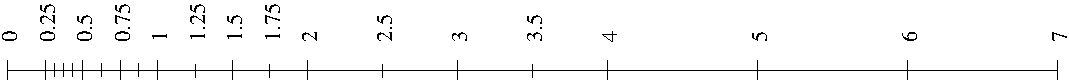
\includegraphics[width=.95\textwidth]{pic/float.pdf}
\end{center}
\caption{Distribution of the floating point numbers. This figure shows a distribution of a sample floating point number set with a precision $t=3$, and $e_{min}=-1$ and $e_{max}=3$.}
\label{fig.float}
\end{figure}


There are two basic floating point \index{Floating point} data types \index{Floating point!Data types}, as defined by the IEEE 754-2008 \cite{ieee754} standard, are shown in \tabref{tab.floatingpointdatatypes}.

\begin{table}[htb]
\begin{center}
\begin{tabular}{|r|c|c|c||c||c|}
% Draw horizontal table line from column 2 to column 6
% The first column is left empty, without the horizontal line
\cline{2-6}

% Since we do not want to change the formatting of the first column
% we need to use the multicolumn macro \multicolumn{#ofcolumns}{newformatting}{content}
% so we can change |r| to just r|. If we did not do that, we'd have the left
% vertical line drawn in the first column. Also in order to make the header row
% nicer, we use the \vrule macro. See below for an explanation.
\multicolumn{1}{r|}{} & {\vrule height 13pt depth 6pt width 0pt\textbf{Sign}} [b] & \textbf{Exponent} [b] & \textbf{Mantissa} [b] & \textbf{Prec.} [dig] & \textbf{Total} [b]\\ \cline{2-6}  \hline

% This vrule shows that we can extend the column height or depth if necessary.
% This is useful for header rows or rows that contain some mathematical expressions.
\vrule height 10pt depth 20pt width 0pt
\textbf{binary32}   			& 1    & 8        	& 24      & 8  	& 32\\ \hline

% To debug, make the vertical rule visible by specifying its width to 1 pt rather than 0 pt.
\vrule height 20pt depth 0pt width 1pt
\textbf{binary64}   			& 1    & 11       	& 53      & 16	& 64\\ \hline
\end{tabular}
\end{center}
\caption{Basic floating point data types.}
\label{tab.floatingpointdatatypes}
\end{table}

\chapter{Main Results}
\label{chap.mainresults}
% If you have a lot of results, feel free to split this chapter into two or more chapters.

\section{Main Result 1}

\section{Main Result 2}

\section{Main Result 3}

\begin{theorem}
    Some theorem\dots
\end{theorem}

\begin{proof}
    Its proof\dots
\end{proof}


\begin{corollary}
    The corollary is\dots
\end{corollary}

\section{Discussion}

\section{Summary}

\widowpenalty=9999
\chapter{Conclusions}
% Summarize each chapter in one paragraph, point out the most important findings.
% 
\section{Summary}

\section{Contributions of the Dissertation Thesis}


\section{Future Work}
% Suggest the possible future work and your recommendations
The author of the \thesis{} suggests to explore the following:
\begin{itemize}
\item It would be interesting to \dots

\item Consider \dots

\item The implementation of our methodology could be further improved \dots

\item Apply the \dots

\item \dots
\end{itemize}
%------------------------------------------------------------------------------------------
% Use bibtex to produce bibliography used in the thesis, except for your own publications
%------------------------------------------------------------------------------------------
\bibliographystyle{plainurl}
%\bibliographystyle{abbrv}
% \cleardoublepage\phantomsection\addcontentsline{toc}{chapter}{\protect\numberline{}{Bibliography}}
\bibliography{main}

% list your own books or papers in refereed journals or conference proceedings
% or chapters in scientific monographies that are RELEVANT FOR YOUR THESIS
\newcounter{MyPublRefCount}
\setcounter{MyPublRefCount}{0}
\def\bibauthor#1{\addtocounter{MyPublRefCount}{1}\bibitem[A.\theMyPublRefCount]{#1}}
\renewcommand\bibname{Reviewed Publications of the Author Relevant to the Thesis}
% \cleardoublepage\phantomsection\addcontentsline{toc}{chapter}{\protect\numberline{}{Reviewed Relevant Publications of the Author}}
\begin{thebibliography}{A.9}%here fill-in the longest label in the list of your publications
\itemsep=0pt
%
%----------------------------------------------------
% \bibauthor{ID}. Cite as \cite{ID}.
\bibauthor{YOURPUBL-ZZZ1}
Gortz, R.; T\"ol\"ok\"o, F.
\newblock On the Carpathian Castle.
\newblock In: \textit{Transylvanian Journal of \dots}.
\newblock Werst, Romania,
\newblock 2010.
% nepovinny blok s citaci:
% ************* 
\bigskip \\ \smallskip The paper has been cited in:
\begin{itemize}
\item Nov\'ak\r{u}, \v{S}. Carpathian Castle Revealed. \textit{International Symposium on Carpathian Legends}. 1:319--323, 2010.
\end{itemize}
% *************
\end{thebibliography}

\renewcommand\bibname{Remaining Publications of the Author Relevant to the Thesis}
% \cleardoublepage\phantomsection\addcontentsline{toc}{chapter}{\protect\numberline{}{Remaining Relevant Publications of the Author}}
\begin{thebibliography}{A.9}%here fill-in the longest label in the list of your publications
%----------------------------------------------------
\bibauthor{YOURPUBL-MINIMUM}
Gortz, R.
\newblock \textit{MINIMUM TITLE}.
\newblock Ph.D. Minimum Thesis, Faculty of Information Technology,
\newblock Prague, Czech Republic,
\newblock 2010.
% nepovinny blok s citaci:
% ************* 
\bigskip \\ \smallskip The paper has been cited in:
\begin{itemize}
\item L\'ef\`evre, \c{C}. \textit{Le Ch\^ateau des Carpathes : Le fin alternatif d\'ecouvert~!}, \dots.
\item Q. Ma\~nana. \dots
\item H. Erd\H{o}s. \dots
\item \r{A}. S\o renson. \dots

\end{itemize}
% *************
\end{thebibliography}

\renewcommand\bibname{Remaining Publications of the Author}
% \cleardoublepage\phantomsection\addcontentsline{toc}{chapter}{\protect\numberline{}{Remaining Publications of the Author}}
\begin{thebibliography}{A.9}%here fill-in the longest label in the list of your publications
%----------------------------------------------------
\bibauthor{YOURPUBL-P2}
Gortz, R.
\newblock Another publication.
\newblock \textit{36\textsuperscript{th} International Conference on \dots}. pp. 19--24, \v{S}trbsk\'e pleso, Slovak Republic,
\newblock 2010.
%*************************************************************************
\end{thebibliography}

\appendix

\appendix
\chapter{Some appendix}
\label{app.1}
\section{\dots}
\section*{Section not in the Table of Contents}

% % Add the index if it is requested above
% \ifx\printindex\undefined\relax\else\cleardoublepage\phantomsection\addcontentsline{toc}{chapter}{\protect\numberline{}{Index}}\fi
% \ifx\printindex\undefined\relax\else\printindex\fi
\end{document}
